% 中文校对稿，仅供作者核对，不用于期刊投稿。
\documentclass[largeformat]{interact}

\usepackage{fontspec}
\usepackage{xeCJK}
\setmainfont{TeX Gyre Termes}
\setCJKmainfont[AutoFakeSlant=0.2]{Noto Serif CJK SC}
\setCJKsansfont{Noto Sans CJK SC}
\setCJKmonofont{Noto Sans Mono CJK SC}
\usepackage{amsmath,amssymb,amsthm}
\usepackage{booktabs,array}
\usepackage{graphicx}
\usepackage{xcolor}
\usepackage[caption=false]{subfig}
\usepackage{adjustbox}
\usepackage[ruled,vlined,linesnumbered]{algorithm2e}
\usepackage[natbibapa]{apacite}
\setlength\bibhang{12pt}
\renewcommand\bibliographytypesize{\fontsize{10}{12}\selectfont}
\usepackage[hidelinks,unicode]{hyperref}
\usepackage{microtype}

\renewcommand{\doi}[1]{\href{https://doi.org/#1}{https://doi.org/#1}}
\graphicspath{{figures/}{figures/dreamview/}}

\definecolor{deepblue}{RGB}{0,114,178}
\definecolor{lightblue}{RGB}{187,220,238}
\definecolor{skyblue}{RGB}{86,180,233}
\definecolor{inputyellow}{RGB}{240,228,66}
\definecolor{outputpink}{RGB}{204,121,167}
\definecolor{improvedpink}{RGB}{213,94,0}
\definecolor{lightpink}{RGB}{230,159,0}
\definecolor{deeppink}{RGB}{213,94,0}
\definecolor{bglight}{RGB}{244,244,244}
\definecolor{lightgreen}{RGB}{0,158,115}
\definecolor{lightorange}{RGB}{230,159,0}
\definecolor{dangerred}{RGB}{213,94,0}
\definecolor{vibrantgreen}{RGB}{0,158,115}
\definecolor{vibrantorange}{RGB}{230,159,0}
\definecolor{vibrantred}{RGB}{213,94,0}

\theoremstyle{plain}
\newtheorem{theorem}{定理}[section]
\newtheorem{lemma}[theorem]{引理}
\newtheorem{proposition}[theorem]{命题}

\DontPrintSemicolon
\SetAlgoCaptionSeparator{。}
\SetAlgorithmName{算法}{算法}{算法目录}
\SetKwInput{KwIn}{输入}
\SetKwInput{KwOut}{输出}
\SetKw{Return}{返回}
\renewcommand{\abstractname}{摘要}
\renewcommand{\keywordsname}{关键词}
\renewcommand{\figurename}{图}
\renewcommand{\tablename}{表}
\renewcommand{\refname}{参考文献}
\providecommand{\pp}{百分点}
\providecommand{\MIKU}{MIKU}
\providecommand{\code}[1]{\texttt{#1}}

\articletype{研究论文}
\received{中文校对稿，非投稿版本}
\title{动态多障碍交通中的交互感知时空同伦约束路径—速度规划}
\author{%
  \name{JiaWang Liao\textsuperscript{a}, YuFei Hu\textsuperscript{a}, ChaoYang Shi\textsuperscript{a} and ChengJiao Sun\textsuperscript{a}\thanks{通讯作者：ChengJiao Sun。邮箱：jiao1952@126.com}}
  \affil{\textsuperscript{a}湖北文理学院计算机工程学院，湖北省襄阳市隆中路296号，邮政编码441053}}
\hypersetup{pdftitle={动态多障碍交通中的交互感知时空同伦约束路径—速度规划},pdfauthor={JiaWang Liao, YuFei Hu, ChaoYang Shi, ChengJiao Sun}}

\begin{document}
\maketitle
\enlargethispage{8pt}

\begin{abstract}
路径—速度分解有利于高效规划，但可能丢失交互时序信息。无时间意识的路径边界会把不同时间发生的占用合并，逐障碍物的侧向选择还可能产生相互冲突的阻塞。本文提出多障碍交互感知运动学约束统一方法 MIKU。该方法保留下游路径二次规划和速度二次规划，通过依赖到达时间的投影避免合并时间上不相交的占用，通过威胁感知裕度和连续划分生成群组级横向带，并利用时空同伦图将安全通行时间窗编译为站位—时间盒约束。在固定截面区间模型下，最大间隙扫描将 $k$ 个障碍物的侧向分配搜索从 $O(2^k)$ 降为 $O(k\log k)$，并在 4,000 个确定性区间实例上与穷举结果一致。在覆盖七类交通构型的 3,500 个配对仿真场景中，MIKU 将无碰撞到达目标率从 62.7\% 提高到 77.5\%，差值为 14.8 个百分点，95\% 置信区间为 13.5--16.0，并将碰撞率从 2.2\% 降至 1.1\%，平均进度提高 8.9 个百分点。规划时间的中位数和第 95 百分位分别为 9.98 ms 和 55.93 ms，但第 99 百分位为 221.8 ms，高于基线的 138.9 ms。独立的 700 场景滚动重规划实验和 Apollo 11.0 接口案例支持重规划行为与软件接入判断，但不构成道路测试。结果表明，在不替换既有凸优化器的前提下，在约束接口处保留交互时序能够减少不必要的停车，但仍需接受尾部延迟和仿真到道路验证的限制。
\end{abstract}

\begin{keywords}
自动驾驶；路径—速度分解；时空同伦；动态障碍物；运动规划
\end{keywords}

\section{引言}
\label{zh:sec:introduction}

自动驾驶车辆需要在动态交通中持续前进，同时满足碰撞规避和乘坐舒适性要求。因此，过度保守的运动规划并非没有代价。反复触发的兜底停车会降低服务可靠性、阻碍周围交通，并削弱智能交通系统应有的机动性收益。运动规划综述因此通常将可行性、安全性、舒适性和计算代价视为相互耦合的运营结果，而不是可以相互替代的单一指标 \citep{gonzalez2016,paden2016,schwarting2018planning}。

路径—速度分解（path--velocity decomposition，PVD）适合在线运行，因为它在站位—横向（station--lateral，SL）坐标中生成横向路径，在站位—时间（station--time，ST）坐标中优化纵向速度 \citep{kant1986pvd,werling2010,zhou2021dliaps}。工业实现由此可以求解两个结构化二次规划（quadratic program，QP），并通过路径边界和 ST 边界向求解器传递环境信息 \citep{fan2018baidu,zhou2021pathqp,wang2022_jfr}。然而，这种分解也可能丢失密集动态场景所需要的关键信息。由当前时刻快照或整个预测时域的并集构成的路径边界，无法区分某一区域是当前被占用，还是在自车到达时已经空闲。此外，逐障碍物做出的不可逆侧向选择，可能以互不兼容的方式抬高路径下界并压低路径上界，即使联合选择后仍存在可通行的通道。

联合时空搜索、混合整数优化和走廊方法可以协调这些决策，但通常需要替换原有求解器、扩大状态空间，或反复调用路径和速度阶段 \citep{mcnaughton2011lattice,kessler2023,yoon2024stcorridor}。本文考察的是另一种可能性，即能否在已有 PVD 栈的约束接口处恢复丢失的交互信息。本文提出的多障碍交互感知运动学约束统一方法（Multi-obstacle Interaction-aware Kinematic constraint Unification，MIKU）构造随时间变化的横向带，选择空间和时间同伦类别，并将其编译为两个 QP 已经支持的盒约束。

本文围绕以下四个研究问题展开：
\begin{enumerate}
  \item[RQ1.] 与匹配的 PVD 基线相比，交互感知约束构造在多大程度上能够改善无碰撞到达目标和交通进度。
  \item[RQ2.] 哪些空间、时间和不确定性处理组件造成了观测到的效果。
  \item[RQ3.] 在哪些运行条件下，鲁棒性、舒适性或计算代价会限制方法收益。
  \item[RQ4.] 在不改变下游 QP 结构的情况下，同一约束接口能否接入已有的 PVD 软件栈。
\end{enumerate}

\begin{figure}
\centering
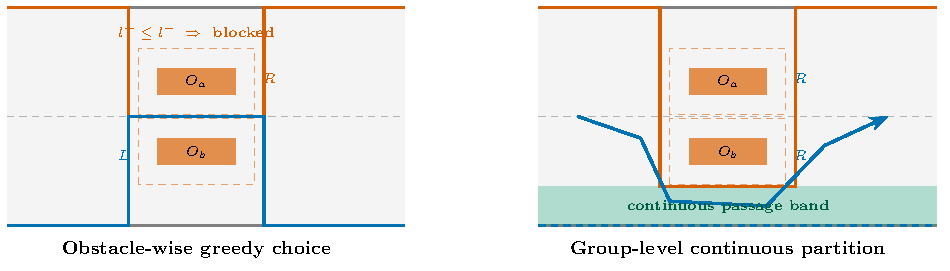
\includegraphics[width=\textwidth]{fig_teaser_en.pdf}
\caption{MIKU 针对的失效模式。即使群组级连续通道仍然存在，独立的侧向选择也可能使路径下界和上界相互穿越。图内变量和模块名称保留英文，以便与实现对应。}
\label{zh:fig:teaser}
\end{figure}

本文的主要贡献如下。
\begin{enumerate}
  \item 在中心坐标边界中形式化了依赖到达时间的 SL 投影和群组级障碍物侧向分配。连续划分引理将 $k$ 个活动障碍物的 $2^k$ 种分配缩减为 $k+1$ 个候选点，并在固定截面区间模型下通过 $O(k\log k)$ 最大间隙扫描确定最宽横向带。
  \item 通过不确定性扩展占用管、可安全通行时间窗和分层时间同伦图，将空间决策连接到速度规划。选定的时序条件仍然表现为线性 ST 盒约束，因此保留下游路径 QP 和速度 QP 的目标函数、运动学等式、凸性及稀疏结构。
  \item 通过匹配的证据链检验每项主张，包括 4,000 个确定性区间检查、带置信区间和组件消融的 3,500 个配对场景、独立的 700 场景滚动重规划实验、有限网格联合参考以及三个 Apollo 11.0 接口案例。分析在报告收益的同时，也报告不利的尾部延迟和依赖条件的权衡。
\end{enumerate}

第~\ref{zh:sec:related_work} 节将约束接口方法置于联合规划器和分解式规划器之间进行定位。第~\ref{zh:sec:problem} 节定义 PVD 接口及其两种失效机制。第~\ref{zh:sec:method} 节介绍 MIKU，第~\ref{zh:sec:experimental_design} 节和第~\ref{zh:sec:results} 节说明评估设计与结果，第~\ref{zh:sec:discussion}--\ref{zh:sec:conclusion} 节讨论工程含义、局限和结论。

\section{相关工作}
\label{zh:sec:related_work}

\subsection{联合时空规划}

联合规划器通过搜索或优化扩展状态保留几何和时间耦合。共形时空格栅直接协调位置、速度和时间 \citep{mcnaughton2011lattice}。瞬时分析方法以及 SLT 形式化方法也在密集交通中联合处理横向和纵向决策 \citep{yang2021_ia_planner,hu2023_hybrid_astar_slt,hu2025_dp_nmpc,qiao2025stjoint}。混合整数形式化则可以用离散变量编码障碍物侧向选择 \citep{kessler2023}。这些方法具有较强的协调能力，但其扩大的搜索空间、整数决策或非线性规划结构，与许多 PVD 栈使用的两个串联凸 QP 存在结构差异。因此，本文后续使用的有限网格联合搜索只作为计算参考，不将其声称为连续问题的最优解。

\subsection{分解式与迭代式协调}

PVD 规划器先优化路径，再优化速度轮廓，从而获得计算可处理性 \citep{kant1986pvd,werling2010}。凸平滑和分段加加速度优化使这种结构适用于面向生产的软件 \citep{fan2018baidu,zhou2021dliaps,zhou2021pathqp}。时间优化、迭代锚定、候选配对和风险感知协调能够在两个阶段之间回传信息 \citep{liu2017speed,chen2019em,zhang2023_dp_rcg,han2026_contingency,pathspeedstructured2024}。但它们的有效性取决于每个阶段暴露了哪些信息。反复更新到达时间，无法恢复已经被不可逆局部侧向决策丢弃的横向类别。

安全走廊方法在连续优化之前显式给出可行域。空间飞行走廊展示了凸集如何连接离散搜索和轨迹优化 \citep{liu2017sfc}，近期自动驾驶研究又将这一思想扩展到时空换道走廊或 Frenet 走廊 \citep{yoon2024stcorridor,frenetcorridor2025}。MIKU 同样强调显式可行域，但关注更窄的接口问题，即如何在不替换路径 QP 和速度 QP 的情况下，生成相互一致的 SL 边界与 ST 边界。

\subsection{交互预测与安全裕度}

预测感知规划能够处理静态障碍物轮廓无法表达的行人和车辆交互 \citep{yangbo2023ped,jeong2021ml}。这类预测仍然存在不确定性，因此规划器需要区分用于估计到达时刻的名义状态和用于碰撞检查的占用集合。MIKU 使用前者查询并排序候选方案，同时用有界的位置误差和速度误差扩展后者。进一步的威胁相关附加裕度按照碰撞紧迫性、横向重叠、相对运动、目标类型和局部密度分配有限的横向空间，其中碰撞时间仅作为一个归一化紧迫性因子 \citep{minderhoud2001extended}。

表~\ref{zh:tab:method_classes} 从求解器层面总结了这些差异。已有方法在各自假设下都具有价值，但仍缺少一种 PVD 栈，能够在保留下游 QP 的同时，联合协调依赖时间的投影、群组级侧向选择以及速度阶段的时序约束。

\begin{table}
\tbl{规划方法族与约束接口问题的关系。}{%
\small
\begin{tabular}{p{0.18\textwidth}p{0.24\textwidth}p{0.23\textwidth}p{0.25\textwidth}}
\toprule
方法族 & 时空协调方式 & 对求解器的影响 & 本文所处理的接口缺口 \\
\midrule
无时间意识的 PVD & 先路径后速度 & 两个结构化 QP & 丢失依赖到达时刻的占用信息和群组选择 \\
迭代式 PVD & 反复更新路径与速度 & 多次调用求解器 & 仅靠时序无法恢复已丢弃的横向类别 \\
联合格栅或混合整数规划 & 耦合状态或离散变量 & 扩大搜索或更换优化器 & 不保留原有的双 QP 接口 \\
安全走廊规划 & 优化前构造凸可行集 & 走廊生成器加连续求解器 & 往往只关注选定走廊，而非耦合的空间和时间类别 \\
MIKU & 将空间和时间同伦编译为边界 & 保留两个下游 QP & 处理到达时序、群组决策和跨阶段约束传递 \\
\bottomrule
\end{tabular}}
\label{zh:tab:method_classes}
\end{table}

\section{问题形式化与证据范围}
\label{zh:sec:problem}

\subsection{路径—速度接口}

考虑与道路对齐的 Frenet 坐标系，其中 $s$ 表示站位，$l$ 表示相对于参考线的横向位移。PVD 规划器首先在 SL 空间中优化横向路径 $l(s)$，随后在 ST 空间中优化纵向运动 $s(t)$。令路径状态为 $\mathbf{x}_p=(l_j,l'_j,l''_j)_{j=0}^{K}$，速度状态为 $\mathbf{x}_v=(s_r,v_r,a_r)_{r=0}^{N}$，则常见的下游求解器可写为
\begin{align}
 \mathbf{x}_p^*={}&\arg\min_{\mathbf{x}_p}
 \frac{1}{2}\mathbf{x}_p^{\mathsf T}H_p\mathbf{x}_p+q_p^{\mathsf T}\mathbf{x}_p,\\[-2pt]
 &\quad\text{s.t. }A_p\mathbf{x}_p=b_p,\quad l_j^-\leq l_j\leq l_j^+, \label{zh:eq:path_qp}\\
 \mathbf{x}_v^*={}&\arg\min_{\mathbf{x}_v}
 \frac{1}{2}\mathbf{x}_v^{\mathsf T}H_v\mathbf{x}_v+q_v^{\mathsf T}\mathbf{x}_v,\\[-2pt]
 &\quad\text{s.t. }A_v\mathbf{x}_v=b_v,\quad s_r^{lb}\leq s_r\leq s_r^{ub},\\[-2pt]
 &\qquad 0\leq v_r\leq v_{\max},\quad a_{\min}\leq a_r\leq a_{\max}. \label{zh:eq:speed_qp}
\end{align}
其中，$H_p$ 和 $H_v$ 编码平滑性代价，$A_p$ 和 $A_v$ 编码分段加加速度运动学等式。路径边界集合 $\mathcal{B}_l=\{[l_j^-,l_j^+]\}$ 与 ST 位置边界集合 $\mathcal{B}_s=\{[s_r^{lb},s_r^{ub}]\}$ 是环境信息的接口。MIKU 只改变这两个接口，不改变下游目标矩阵、运动学等式和 QP 求解器。

\subsection{中心坐标障碍物模型}

对于障碍物 $i$，令 $O_i(t)=[s_i^-(t),s_i^+(t)]\times[l_i^-(t),l_i^+(t)]$ 表示其物理矩形。若道路物理边界为 $[l_{\mathrm{road}}^-,l_{\mathrm{road}}^+]$，自车宽度为 $W_{\mathrm{ego}}$，路侧裕度为 $d_{\mathrm{road}}$，则自车中心的可行区间为
\begin{equation}
 [L^-,L^+]=[l_{\mathrm{road}}^-+W_{\mathrm{ego}}/2+d_{\mathrm{road}},\ l_{\mathrm{road}}^+-W_{\mathrm{ego}}/2-d_{\mathrm{road}}].
 \label{zh:eq:center_road}
\end{equation}
传递给中心坐标规划器的障碍物区间会一次性扩展自车宽度的一半以及障碍物特定的附加裕度 $d_{\mathrm{buf},i}$：
\begin{equation}
 [u_i,v_i]=[l_i^- -W_{\mathrm{ego}}/2-d_{\mathrm{buf},i},\ l_i^+ +W_{\mathrm{ego}}/2+d_{\mathrm{buf},i}].
 \label{zh:eq:center_forbidden}
\end{equation}
式~(\ref{zh:eq:center_road})--式~(\ref{zh:eq:center_forbidden})中的四个量均指自车中心。因此，间隙宽度表示中心位置可用的宽度，后续可行性测试不再重复减去车辆宽度。

在某一站位处的 $k$ 个活动障碍物集合中，将每个障碍物分配到自车带的左侧（$L$）或右侧（$R$）。对于决策向量 $\mathbf{d}$，得到的中心带为
\begin{equation}
 l^-(\mathbf{d})=\max\left(L^-,\max_{i\in\mathcal{L}}v_i\right),\qquad
 l^+(\mathbf{d})=\min\left(L^+,\min_{i\in\mathcal{R}}u_i\right),
 \label{zh:eq:center_band}
\end{equation}
其中空集合的极值项省略。当数值容差为 $\varepsilon$ 时，若 $W(\mathbf{d})=l^+(\mathbf{d})-l^-(\mathbf{d})\geq\varepsilon$，则该中心带可行。

\subsection{两种失效机制与研究边界}

当路径阶段忽略时间时，可能用预测时域上的并集替代动态占用
\begin{equation}
 \overline{O}_i=\bigcup_{t\in[0,T_{\mathrm{pred}}]}O_i(t),
 \label{zh:eq:prob_union}
\end{equation}
从而把不同时间被占用的位置当成同时存在。相反，逐障碍物的贪心策略可能在尚未看到同一纵向连通分量中另一个障碍物影响之前，就提前确定侧向。两种机制都可能造成 $l^+(s)<l^-(s)$，即使从时间上保持一致的通道仍然存在。

本文检验的是，在边界接口处恢复缺失的到达时间信息和群组级信息，是否能够改善规划结果。主要证据来自直道路段、恒定速度障碍物模型和有界扰动场景。3,500 个场景实验是匹配的数值评估，不是公共数据或道路现场研究。Apollo Planning 仅用于接口和代表性行为证据，不将其视为物理道路测试或 Apollo 原生运行时间基准。

\section{MIKU 方法}
\label{zh:sec:method}

\subsection{总体流程}

MIKU 重建无时间意识的 PVD 和逐障碍物 PVD 所丢失的两类信息。首先估计自车到达时间 $\tau(s)$，并查询依赖时间的障碍物占用。随后计算依赖威胁的中心边界，对纵向连通的障碍物进行分组，并选择连续的横向带。在路径 QP 求解之后，用不确定性扩展的占用管定义安全通行时间窗。分层时间同伦图选择具有因果一致性的时间窗序列，并将其写入 ST 位置边界。图~\ref{zh:fig:miku_flow} 总结了数据流。

\begin{figure}
\centering
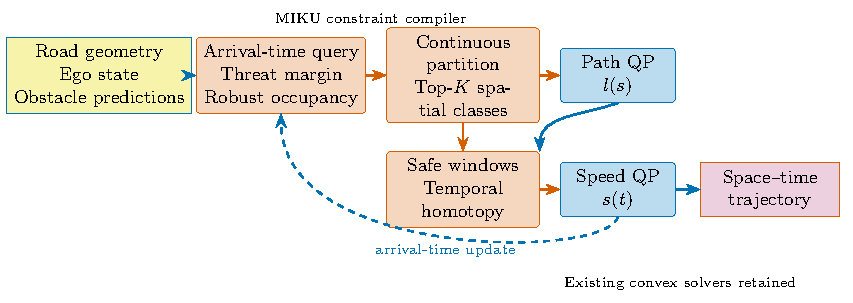
\includegraphics[width=\textwidth]{fig_framework_en.pdf}
\caption{MIKU 在 PVD 规划栈中的约束构造与传递。图内模块和变量名称保留英文，以便与实现对应。}
\label{zh:fig:miku_flow}
\end{figure}

\subsection{威胁感知裕度}
\label{zh:sec:method_threat}

对于障碍物 $i$，MIKU 将碰撞紧迫性、横向重叠、相对运动、目标类型和局部交互密度组合为归一化威胁分数：
\begin{equation}
 \Theta_i=w_1f_{\mathrm{TTC}}(i)+w_2f_{\mathrm{overlap}}(i)+w_3f_{\mathrm{vel}}(i)+w_4f_{\mathrm{type}}(i)+w_5f_{\mathrm{inter}}(i).
 \label{zh:eq:threat_score}
\end{equation}
所有因子均位于 $[0,1]$，权重为 $(0.30,0.20,0.15,0.10,0.25)$。当自车位于障碍物后方且正在接近时，$\mathrm{TTC}_i=(s_i-s_{\mathrm{ego}})/(\dot{s}_{\mathrm{ego}}-\dot{s}_i)$，否则取 $+\infty$。分段线性 TTC 因子在 $\mathrm{TTC}_i\leq2.0$ s 时取 1，在 $\mathrm{TTC}_i\geq7.0$ s 时取 0，中间区间线性下降 \citep{minderhoud2001extended}。重叠因子和相对速度因子为
\begin{align}
 f_{\mathrm{overlap}}(i)&=\min\!\left(1,\frac{\max(0,\min(l_i^+,l_{\mathrm{ego}}^+)-\max(l_i^-,l_{\mathrm{ego}}^-))}{\max(0.1,\min(W_i,W_{\mathrm{ego}}))}\right),\\
 f_{\mathrm{vel}}(i)&=\sigma(v_{\mathrm{rel},i}/v_{\max}),\qquad \sigma(x)=\frac{1}{1+e^{-5x}}.
\end{align}
其中 $W_i=l_i^+-l_i^-$ 表示障碍物宽度。截断操作使障碍物宽于自车时的重叠因子仍处于 $[0,1]$。易受伤道路使用者、机动车、未知可移动物体、静态障碍物和小型标记物的类型因子分别为 $1.0$、$0.7$、$0.5$、$0.3$ 和 $0.15$。密度在 10 m 邻域内计算，单个障碍物的密度取 0。附加裕度为
\begin{equation}
 d_{\mathrm{buf},i}=d_{\mathrm{buf,min}}+(d_{\mathrm{buf,max}}-d_{\mathrm{buf,min}})\Theta_i,
 \label{zh:eq:dynamic_delta}
\end{equation}
其中 $[d_{\mathrm{buf,min}},d_{\mathrm{buf,max}}]=[0.10,0.40]$ m。该项只改变边界数值，不改变排序或扫描结构。

\subsection{连续横向划分与最大间隙}
\label{zh:sec:method_band}

纵向区间相互重叠的障碍物被分配到同一个连通分量。按较低站位边缘排序，并维护最大的上界，即可在 $O(n\log n)$ 时间内构造所有分量。在一个分量内部，再按 $u_i$ 对活动区间排序，$u_i$ 相同时按 $v_i$ 降序排列。下面的引理限制侧向分配搜索范围。

\begin{lemma}[连续最优划分]
\label{zh:lem:continuous_partition}
对于式~(\ref{zh:eq:center_band})中的中心带目标，存在一个最优分配，使得按 $u_i$ 排序的障碍物中，前缀被分配到 $L$ 侧，后缀被分配到 $R$ 侧。因此只需考察 $k+1$ 个分割点。
\end{lemma}

\emph{证明。} 若两侧均非空，令 $\beta=\min_{i\in\mathcal{R}}u_i$。将当前位于 $\mathcal{L}$ 且满足 $u_i\geq\beta$ 的每个障碍物移到 $\mathcal{R}$。由于每个被移动的下边缘都不小于 $\beta$，上界保持不变，而从 $\mathcal{L}$ 中移除元素不会抬高下界，因此带宽不会减小。重复该操作即可得到连续分割。空侧情况对应 $p=0$ 或 $p=k$。对于 $u_i$ 相同的情况按 $v_i$ 降序排列即可消除歧义。\hfill$\Box$

对于分割点 $p$，定义前缀最大值和候选上边缘
\begin{equation}
 V_0=L^-,\qquad V_p=\max\left(L^-,\max_{1\leq q\leq p}v_{(q)}\right),
 \label{zh:eq:prefix_v}
\end{equation}
\begin{equation}
 U_p=\begin{cases}\min(L^+,u_{(p+1)}),&p<k,\\L^+,&p=k,\end{cases}\qquad g_p=U_p-V_p.
 \label{zh:eq:gap_def}
\end{equation}

\begin{theorem}[最大间隙最优性]
\label{zh:thm:max_gap}
对于固定截面区间模型，最优中心带宽度为 $W^*=\max_{p=0,\ldots,k}g_p$。候选解通过排序和一次前缀扫描获得，复杂度为 $O(k\log k)$。
\end{theorem}

\emph{证明。} 对于分割点 $p$，式~(\ref{zh:eq:center_band})给出下边缘 $V_p$ 和最紧的上边缘 $U_p$，因此带宽为 $g_p$。引理~\ref{zh:lem:continuous_partition} 保证存在连续最优分割，枚举 $k+1$ 个分割点即可取得最优值。\hfill$\Box$

该定理只对固定截面区间抽象成立，不能证明完整非凸轨迹问题的连续全局最优性。MIKU 在每个分量中保留 $Q=3$ 个最宽的正带，并通过动态规划在带宽与横向中心变化之间进行权衡。若分量 $j$ 中的带 $B_{jq}$ 具有中心 $c_{jq}$ 和宽度 $g_{jq}$，则序列最小化
\begin{equation}
 -\sum_jg_{jq_j}+\lambda_s\left(|c_{1q_1}-l_0|+\sum_{j>1}|c_{jq_j}-c_{j-1,q_{j-1}}|\right),
 \label{zh:eq:spatial_homotopy}
\end{equation}
递推关系为
\begin{equation}
 D_{jq}=-g_{jq}+\min_r\{D_{j-1,r}+\lambda_s|c_{jq}-c_{j-1,r}|\}.
 \label{zh:eq:spatial_dp}
\end{equation}

\begin{figure}
\centering
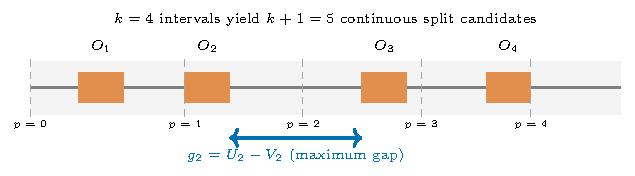
\includegraphics[width=0.82\textwidth]{fig_max_gap_en.pdf}
\caption{固定截面最大间隙问题的连续分割候选。四个排序后的禁行区间产生五个候选分割点。当区间上边缘相互嵌套时，需要维护前缀最大值。图内变量保留英文。}
\label{zh:fig:max_gap}
\end{figure}

\subsection{依赖到达时间的投影}
\label{zh:sec:method_projection}

在站位 $s$ 处，路径阶段查询预计自车到达时刻对应的障碍物占用。根据当前状态并采用恒定加速度近似，有
\begin{equation}
 \tau(s)=\frac{-v_{\mathrm{ego}}+\sqrt{v_{\mathrm{ego}}^2+2a_{\mathrm{ego}}(s-s_{\mathrm{ego}})}}{a_{\mathrm{ego}}},
 \label{zh:eq:arrival_time}
\end{equation}
当 $|a_{\mathrm{ego}}|<10^{-3}$ 时使用恒速极限。判别式为负时，将该点标记为位于规划时域之外。在滚动重规划中，$\tau(s)$ 由上一次速度解插值得到，并在每个周期更新。

数值场景采用 $s_i(t)=s_{i,0}+v_{s,i}t$ 和 $l_i(t)=l_{i,0}+v_{l,i}t$。对于有界预测误差，时刻 $t$ 的纵向和横向扩展为
\begin{equation}
 \epsilon_{s,i}(t)=\epsilon_{s0,i}+t\epsilon_{vs,i},\qquad
 \epsilon_{l,i}(t)=\epsilon_{l0,i}+t\epsilon_{vl,i}.
 \label{zh:eq:prediction_tube}
\end{equation}
在构造 ST 占用图之前，将物理障碍物和自车轮廓按上述量扩展。名义的 $\tau(s)$ 用于选择并排序候选方案，碰撞检查则使用扩展后的占用。

\subsection{时间同伦与 ST 传递}
\label{zh:sec:method_temporal}

对于冲突区域 $c$，令 $I_{cr}=[t_{cr}^{in},t_{cr}^{out}]$ 表示路径与预测占用管之间的每个重叠区间。经过时间安全扩展 $\eta_c$ 后，安全时间窗为
\begin{equation}
 \mathcal{W}_c=[0,T]\setminus\bigcup_r[t_{cr}^{in}-\eta_c,t_{cr}^{out}+\eta_c].
 \label{zh:eq:safe_windows}
\end{equation}
将这些时间窗与最早可到达时间相交，得到 $W_{cq}=[\alpha_{cq},\beta_{cq}]$。对于按站位排序的冲突点，当满足
\begin{equation}
 \hat t_c\geq\hat t_{c-1}+\frac{s_c-s_{c-1}}{v_{\max}},\qquad \hat t_c\in W_{cq}
 \label{zh:eq:temporal_edge}
\end{equation}
时，连接相邻节点。节点代价衡量其与 $\tau(s_c)$ 的偏离，边代价抑制在障碍物前后通行之间进行不必要的切换。带宽受限的动态规划选择一条具有因果关系的序列。

对于选定的时间窗，其语义以线性盒约束进入速度 QP：
\begin{equation}
 \begin{aligned}
 s_j^{ub}&=\min(s_j^{ub,0},s_c^- -\epsilon_s),&&t_j<\alpha_{cq},\\
 s_j^{lb}&=\max(s_j^{lb,0},s_c^+ +\epsilon_s),&&t_j\geq\beta_{cq}.
 \end{aligned}
 \label{zh:eq:window_to_st}
\end{equation}
如果没有完整的可达时间窗序列，规划器会在第一个不可达冲突之前施加停车上界。下游速度 QP 仍然是具有相同目标函数和运动学等式的凸 QP。

\subsection{算法与复杂度}

\begin{algorithm}
\small
\caption{MIKU 约束编译}
\label{zh:alg:miku}
\KwIn{道路边界、自车状态以及 $n$ 个障碍物的预测轨迹}
\KwOut{中心路径边界和 ST 位置边界}
估计 $\tau(s)$，并为每个障碍物计算依赖威胁的中心区间。\;
对站位区间排序并构造纵向连通分量。\;
\ForEach{连通分量}{
  按 $(u_i,-v_i)$ 排序，计算前缀最大值，并保留 $Q$ 个最宽的正带。\;
}
依据式~(\ref{zh:eq:spatial_homotopy})选择连续的空间同伦序列。\;
将选定的侧向分配写入各站位的活动路径边界。\;
构造不确定性扩展的占用管和安全时间窗。\;
依据式~(\ref{zh:eq:temporal_edge})选择具有因果关系的时间同伦序列，并将其编译为式~(\ref{zh:eq:window_to_st})。\;
若启用迭代，则根据速度解更新 $\tau(s)$，直到达到迭代上限或收敛。\;
\Return{路径边界和 ST 边界}
\end{algorithm}

对于 $K$ 个路径采样点、$m$ 个分量、每个分量至多 $Q$ 个空间候选以及有界时间束宽度 $B$，排序和分组的代价为 $O(n\log n)$。若每个终端空间带保留 $K_s$ 个前缀，分层空间动态规划的代价为 $O(mK_sQ^2\log(K_sQ))$。对于 $h$ 个冲突点以及每层 $R$ 个可达时间窗，时间束扩展和排序的代价为 $O(hBR\log(BR))$。实现采用 $Q=3$、$K_s=3$ 和 $B=8$。占用查询的代价为 $O(nK)$，朴素交互密度计算在最坏情况下为 $O(n^2)$。

\section{实验设计}
\label{zh:sec:experimental_design}

实验评估在三个不同层次展开：大规模开环统计仿真、闭环滚动重规划以及在 Apollo Planning 生产架构中的软件集成验证。统计实验使用确定性场景生成器和固定随机种子，使每种方法接收完全相同的环境输入，碰撞与间隙指标则依据独立保留的真实轨迹进行严格评估。

\subsection{实验协议与场景}
\label{zh:sec:protocols_scenarios}

每个场景使用按场景族分配的固定时域 $T\in\{9,10,12,14\}$ s：交叉行人与延迟交叉为 9 s，车辆切入、带对向交通的停放车辆及预测噪声为 10 s，窄间隙多障碍物为 12 s，交错动态障碍物为 14 s。当仿真时钟达到 $T$ 而未达到 $s_{\mathrm{end}}\geq s_{\max}-1$ m 时判为超时。全文使用四套互不重叠的协议。

\emph{开环评估协议，涵盖 3{,}500 个场景。} 七类场景族各使用 500 个随机种子：交叉行人、车辆切入、带对向交通的停放车辆、窄间隙多障碍物、交错动态障碍物、预测噪声与延迟交叉。参数在各场景族范围内采样。除预测噪声场景族仅将有界误差注入规划输入外，规划场景与真实场景完全一致。

\emph{固定截面几何检查，涵盖 4{,}000 个实例。} 20 个确定性随机种子，每个种子生成 200 个固定截面区间实例；每个实例包含 0 到 8 个可能重叠、嵌套或穿越道路边界的禁行区间。扫描算法与全部 $2^k$ 种侧向分配的穷举结果比较中心带宽度。

\emph{滚动重规划评估协议，涵盖 700 个场景。} 每类场景族使用 100 个随机种子。自车在 $t=0$ 时由真实状态 $(s_0,l_0,v_0,a_0)$ 初始化，首个规划周期采用冷启动，不复用 QP 对偶变量的暖启动，也不承继任何同伦决策。每隔 0.5 s 执行当前计划的第一个片段，更新障碍物状态，并在移位后的时域 $\max(2.0\text{ s},T-t)$ 上再次调用规划器，直至自车在 $s\geq s_{\max}-1$ m 到达目标或达到 $T$。

\emph{有限网格联合参考，涵盖 70 个场景。} 分层设置，每类场景族使用 10 个随机种子，网格间距为 $\Delta t=0.5$ s、$\Delta s=0.5$ m、$\Delta l=0.25$ m 与 $\Delta v=1.0$ m/s，束宽设为 20{,}000。

\subsection{基线与实现}
\label{zh:sec:baselines_impl}

匹配的 PVD 基线按照约束接口交换的信息定义：
\begin{itemize}
  \item B0 无时间意识，使用固定的局部侧向策略。
  \item B1 增加依赖到达时间的投影，但保留逐障碍物的贪心侧向选择。
  \item B2 在 B1 策略中允许三次到达时间细化迭代。
  \item MIKU 增加群组级连续划分、Top-$K$ 空间同伦、威胁感知裕度、不确定性扩展占用、时间同伦，以及最多两次交替更新的规划迭代。
\end{itemize}
四种方法共享相同的路径 QP 与速度 QP 目标、运动学约束、输入及指标实现。两个分段加加速度 QP 均在 OSQP 的默认容差下求解，3{,}500 场景运行中不施加逐次调用的墙钟上限。基线 B2 在其三次到达时间细化迭代内使用同一套 QP。基线 B3 是 $(t,s,l,v)$ 网格上的确定性集束搜索动态规划，束宽设为 20{,}000。单步转移代价为相对 $v_0$ 的速度偏差、纵向加速度、横向偏置与横向加速度的加权和再减去进度奖励；运动学不可行或与不确定性扩展障碍物发生碰撞的转移在排序前直接剪除。MIKU 的全部超参数在评估前固定，并汇总于表~\ref{zh:tab:fixed_parameters}。实验运行于配有 64 GB 内存的 Intel i9-14900HX 平台。Apollo 集成验证与 Apollo 11.0 Planning 的兼容性。

\begin{table}[t]
\centering
\caption{全部实验采用的固定规划与预测误差参数}
\label{zh:tab:fixed_parameters}
\small
\begin{tabular}{lll}
\toprule
参数 & 数值 & 用途\\
\midrule
$(w_1,\ldots,w_5)$ & $(0.30,0.20,0.15,0.10,0.25)$ & 威胁度权重\\
TTC 断点 & $2.0,7.0$ s & 紧迫度归一化\\
$(\delta_{\min},\delta_{\max})$ & $(0.10,0.40)$ m & 自适应障碍物缓冲\\
$Q,K_s,\lambda_s$ & $3,3,0.05$ & 空间带、Top-$K$ 与切换权重\\
$B$ & $8$ & 时间图束宽\\
$\eta_c$ & $0.10+0.05\min(|v_l|,2)$ s & 占用时间窗扩展\\
$\epsilon_s$ & $0.05$ m & 纵向 ST 安全裕度\\
$(\epsilon_{s0},\epsilon_{l0})$ & $(0.35,0.18)$ m & 预测位置初始误差界\\
$(\epsilon_{vs},\epsilon_{vl})$ & $(0.30,0.12)$ m/s & 预测误差增长率界\\
路径/速度离散步长 & $0.5$ m / $0.1$ s & QP 采样\\
规划迭代次数 & 最多 $2$ 次 & 初始求解与一次细化\\
\bottomrule
\end{tabular}
\end{table}

\subsection{结果指标与统计分析}
\label{zh:sec:outcomes_stats}

主要结果指标是无碰撞到达目标率：当运行在完整时域内保持无碰撞，并且达到 $s_{\mathrm{end}}\geq s_{\max}-1$ m 时判为成功。碰撞率根据真实矩形评估；退化停车率记录无碰撞但停车或未到达目标的运行。进度比、平均速度、加加速度均方根、最小带符号间隙、最小纵向碰撞时间、带惩罚的行驶时间与规划延迟提供安全性、舒适性与计算方面的背景。无碰撞到达时，带惩罚的行驶时间等于到达时间，否则等于第~\ref{zh:sec:protocols_scenarios} 节中各场景族对应的时域 $T$ 加 5 s。运行时间涵盖完整的方法调用，B2 包括其全部协调迭代。

对于每个固定随机种子，先计算 MIKU 减去基线的差值再行聚合。连续指标使用 5{,}000 次重采样的配对百分位 Bootstrap 区间；二元结果使用精确 McNemar 检验；效应量采用配对 Cohen's $d_z$。运行时间报告第 50、95 与 99 百分位。

\section{结果}
\label{zh:sec:results}

\subsection{基准对比与统计评估}
\label{zh:subsec:results_main}

在定理验证方面，$O(k\log k)$ 扫描与穷举枚举在全部 4,000 个实例上完全一致，中心带宽度的最大差值低于 $10^{-12}$。

在主要配对比较中，表~\ref{zh:tab:main_results} 汇总了 3,500 个配对场景的结果。MIKU 将无碰撞到达目标率从基线 B0 的 62.69\% 提高至 77.46\%，实现配对差值 14.77 个百分点，其 95\% Bootstrap 置信区间为 13.54 至 15.97，精确 McNemar 检验 $p=1.94\times10^{-133}$。碰撞率从 2.17\% 降至 1.14\%，降幅达 1.03 个百分点，95\% 置信区间为 $-1.37$ 至 $-0.71$，$p=2.91\times10^{-11}$。平均进度提高 8.93 个百分点，加加速度均方根降低 0.120 m/s$^3$，带惩罚行驶时间减少 0.81 s。平均间隙的总体差值为 $-0.010$ m，95\% 置信区间为 $[-0.024,0.004]$ m。

\begin{table}
\tbl{3,500 个配对场景基准评估结果。比例以百分数表示，连续指标报告均值，运行时间以毫秒表示。}
{%
\begin{tabular}{lrrrr}
\toprule
指标 & B0 & B1 & B2 & MIKU \\
\midrule
无碰撞到达目标（\%） & 62.69 & 52.37 & 62.09 & \textbf{77.46} \\
碰撞（\%） & 2.17 & 2.14 & 2.23 & \textbf{1.14} \\
退化停车（\%） & 35.40 & 45.77 & 35.97 & \textbf{21.51} \\
进度比（\%） & 77.52 & 71.07 & 76.62 & \textbf{86.45} \\
加加速度均方根（m/s$^3$） & 1.252 & 1.315 & 1.300 & \textbf{1.132} \\
运行时间第 50 百分位（ms） & 10.11 & 11.37 & 31.20 & \textbf{9.98} \\
运行时间第 95 百分位（ms） & 56.79 & 63.24 & 169.49 & \textbf{55.93} \\
运行时间第 99 百分位（ms） & 138.88 & 169.73 & 463.05 & 221.80 \\
\bottomrule
\end{tabular}}
\begin{tabnote}[注]
B0：采用贪心逐障碍物边界的 Apollo 基线；B1：未引入到达时间条件的时间展开占用；B2：3 次迭代启发式耦合；MIKU：本文提出的约束编译器。加粗表示各指标最优结果。所有方法均在 7 类基准场景族相同的初始状态与随机种子下配对评测，样本量 $N=3,500$。
\end{tabnote}
\label{zh:tab:main_results}
\end{table}

在类别层面的效应分析中，图~\ref{zh:fig:evidence_dashboard} 面板 (a) 定位了差异的来源：成功率增益最大的是窄间隙多障碍物类别，提升达 65.4 个百分点；其次是延迟交叉类别，提升达 26.8 个百分点。交叉行人和车辆切入类别未出现总体差异，因为其几何在障碍物任一侧都存在一条主导通道；MIKU 的群组级划分与时间同伦在这些单走廊构型下不改变约束接口，证实该方法在基线接口已经充分的场景中不引入性能退化。预测噪声类别的成功率提高 3.2 个百分点，碰撞率降低 7.0 个百分点；然而进度下降 1.12 个百分点，加加速度均方根上升 0.041 m/s$^3$，这是误差界较大时保守的不确定性扩展占用管的预期副效应。面板 (d) 显示配对增益来自退化停车向成功到达的迁移。

在与联合时空格栅搜索参照 B3 的 70 个案例配对对比中，B3 达到 80.0\%，MIKU 为 77.1\%，配对差值为 $-2.86$ 个百分点，95\% 置信区间为 $[-11.43,5.71]$，$p=0.754$；B3 的运行时间中位数为 1,835.43 ms，而 MIKU 为 10.44 ms。

\begin{figure}
\centering

\includegraphics[width=\textwidth]{evidence_dashboard.pdf}
\caption{3,500 个配对场景的结果汇总。各面板依次给出分场景族成功率差值（a）、规划时延分布（b）、消融降幅（c）与结果构成（d）。}
\label{zh:fig:evidence_dashboard}
\end{figure}

\subsection{组件消融与机制归因}
\label{zh:subsec:results_ablation}

在相同的 3,500 个场景上执行减法消融，沿用第~\ref{zh:sec:experimental_design} 节的 5,000 次重采样 Bootstrap。移除 Top-$K$ 空间同伦后成功率下降 10.17 个百分点；移除威胁感知裕度后下降 10.74 个百分点。移除时间同伦图后，延迟交叉类别成功率从 89.6\% 降至 66.8\%，在该类别上造成 22.8 个百分点的损失。移除鲁棒占用管后，预测噪声类别的碰撞率从 3.6\% 上升至 11.0\%。到达时间投影与纵向分组的总体变化较小，其价值集中于特定构型。图~\ref{zh:fig:evidence_dashboard} 面板 (c) 汇总了下表所列的效应。

\begin{table}
\tbl{相同 3,500 个配对场景上的减法消融结果；$\Delta$ 列给出相对完整 MIKU 的带符号变化，以百分点为单位。}
{%
\begin{tabular}{l lrrrrrr}
\toprule
变体 & 移除组件 & 成功率（\%） & $\Delta$ 成功 & 碰撞率（\%） & $\Delta$ 碰撞 & 进度（\%） & $\Delta$ 进度 \\
\midrule
A1 & 到达时间投影 & 77.34 & $-0.12$ & 1.23 & $+0.09$ & 86.73 & $+0.28$ \\
A2 & 纵向分组 & 76.94 & $-0.52$ & 1.14 & $0.00$ & 85.89 & $-0.56$ \\
A3 & Top-$K$ 空间同伦 & 67.29 & $-10.17$ & 1.14 & $0.00$ & 79.53 & $-6.92$ \\
A4 & 威胁感知裕度 & 66.71 & $-10.74$ & 1.14 & $0.00$ & 78.85 & $-7.60$ \\
A5 & 时间同伦图 & 74.20 & $-3.26$ & 1.17 & $+0.03$ & 84.29 & $-2.16$ \\
A6 & 鲁棒占用管 & 76.97 & $-0.49$ & 2.20 & $+1.06$ & 86.60 & $+0.15$ \\
A7 & 交替细化 & 76.63 & $-0.83$ & 1.03 & $-0.11$ & 85.92 & $-0.53$ \\
MIKU & 无 & \textbf{77.46} & --- & \textbf{1.14} & --- & \textbf{86.45} & --- \\
\bottomrule
\end{tabular}}
\begin{tabnote}[注]
基于相同的 $N=3,500$ 场景并在 5,000 次 Bootstrap 重采样下计算。$\Delta$ 表示相对完整 MIKU 流水线的带符号百分点变化；在成功率或进度上的负 $\Delta$ 以及碰撞率上的正 $\Delta$ 代表移除该组件后系统性能发生退化。加粗表示完整 MIKU 框架。
\end{tabnote}
\label{zh:tab:ablation_results}
\end{table}

几何上，如图~\ref{zh:fig:narrow_mechanism_en}所示，在窄通道中，逐障碍物策略不断抬升与压低相互对置的路径边界，直至中心区间被消解为空；而群组级划分在协调障碍物侧向选择后保留一条连续带。在延迟交叉中，时间图同时保留障碍物前通行与障碍物后通行两条候选，并强制其因果顺序。

\begin{figure}
\centering
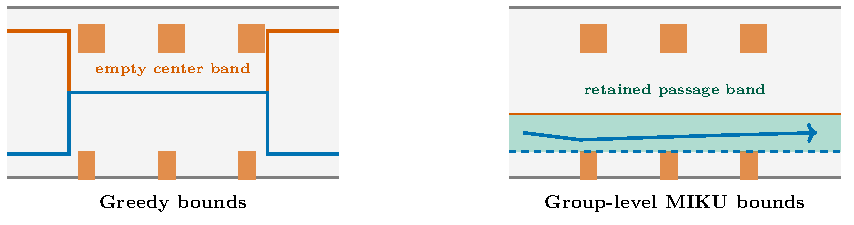
\includegraphics[width=\textwidth]{fig_narrow_en.pdf}
\caption{贪心逐障碍物边界使紧缩处可行区间为空（a）。MIKU 的群组级划分保留连续中心走廊（b）。}
\label{zh:fig:narrow_mechanism_en}
\end{figure}

\subsection{鲁棒性、时延分布与滚动重规划}
\label{zh:subsec:results_robustness}

在预测噪声子组中，除了第~\ref{zh:subsec:results_main} 节报告的 3.2 个百分点成功率增益与 7.0 个百分点碰撞率降低外，MIKU 的平均进度为 59.73\%，B0 为 60.85\%；加加速度均方根为 2.274 m/s$^3$，B0 为 2.234 m/s$^3$。这与如下解释一致：当误差界较大时，不确定性扩展占用会带来较为保守的行为。

完整调用运行时间的中位数与第 95 百分位与 B0 相当或更低，但第 99 百分位并非如此：MIKU 为 221.80 ms，B0 为 138.88 ms，图~\ref{zh:fig:evidence_dashboard} 面板 (b) 中可见上尾的分化。B2 因始终执行三次协调迭代，在所有分位数上都更慢。

滚动重规划协议评估多周期连续规划下的闭环累积控制表现。在 700 个案例中，成功率从 62.29\% 提升至 72.29\%，实现 10.0 个百分点的改善，95\% 置信区间为 7.57 至 12.57；两种方法的碰撞率均为 1.29\%，平均进度从 82.55\% 升至 90.25\%，单回合运行时间第 95 百分位从 827.20 ms 升至 1,361.51 ms。

\subsection{量产软件接口集成与验证}
\label{zh:subsec:results_apollo}

Apollo 11.0 集成直接通过既有的路径边界与 ST 边界模块传递生成的约束条件，完整保留下游 QP 的目标函数、运动学等式与凸优化结构。如图~\ref{zh:fig:apollo_cases}所示，三个代表性 Dreamview 测试工况，即动态超车、窄通道通行与单车道绕行，在 Apollo 0.5\,s 规划周期内均实现了平滑轨迹生成与稳健避障，证实了方法与量产级自动驾驶系统架构的工程兼容性与可行性。

\begin{figure}
\centering
\begin{minipage}{0.32\textwidth}\centering
\includegraphics[width=\linewidth]{dreamview/scn01_during.png}\par\vspace{2pt}\footnotesize (a) 动态超车\end{minipage}\hfill
\begin{minipage}{0.32\textwidth}\centering
\includegraphics[width=\linewidth]{dreamview/scn02_during.png}\par\vspace{2pt}\footnotesize (b) 窄通道通行\end{minipage}\hfill
\begin{minipage}{0.32\textwidth}\centering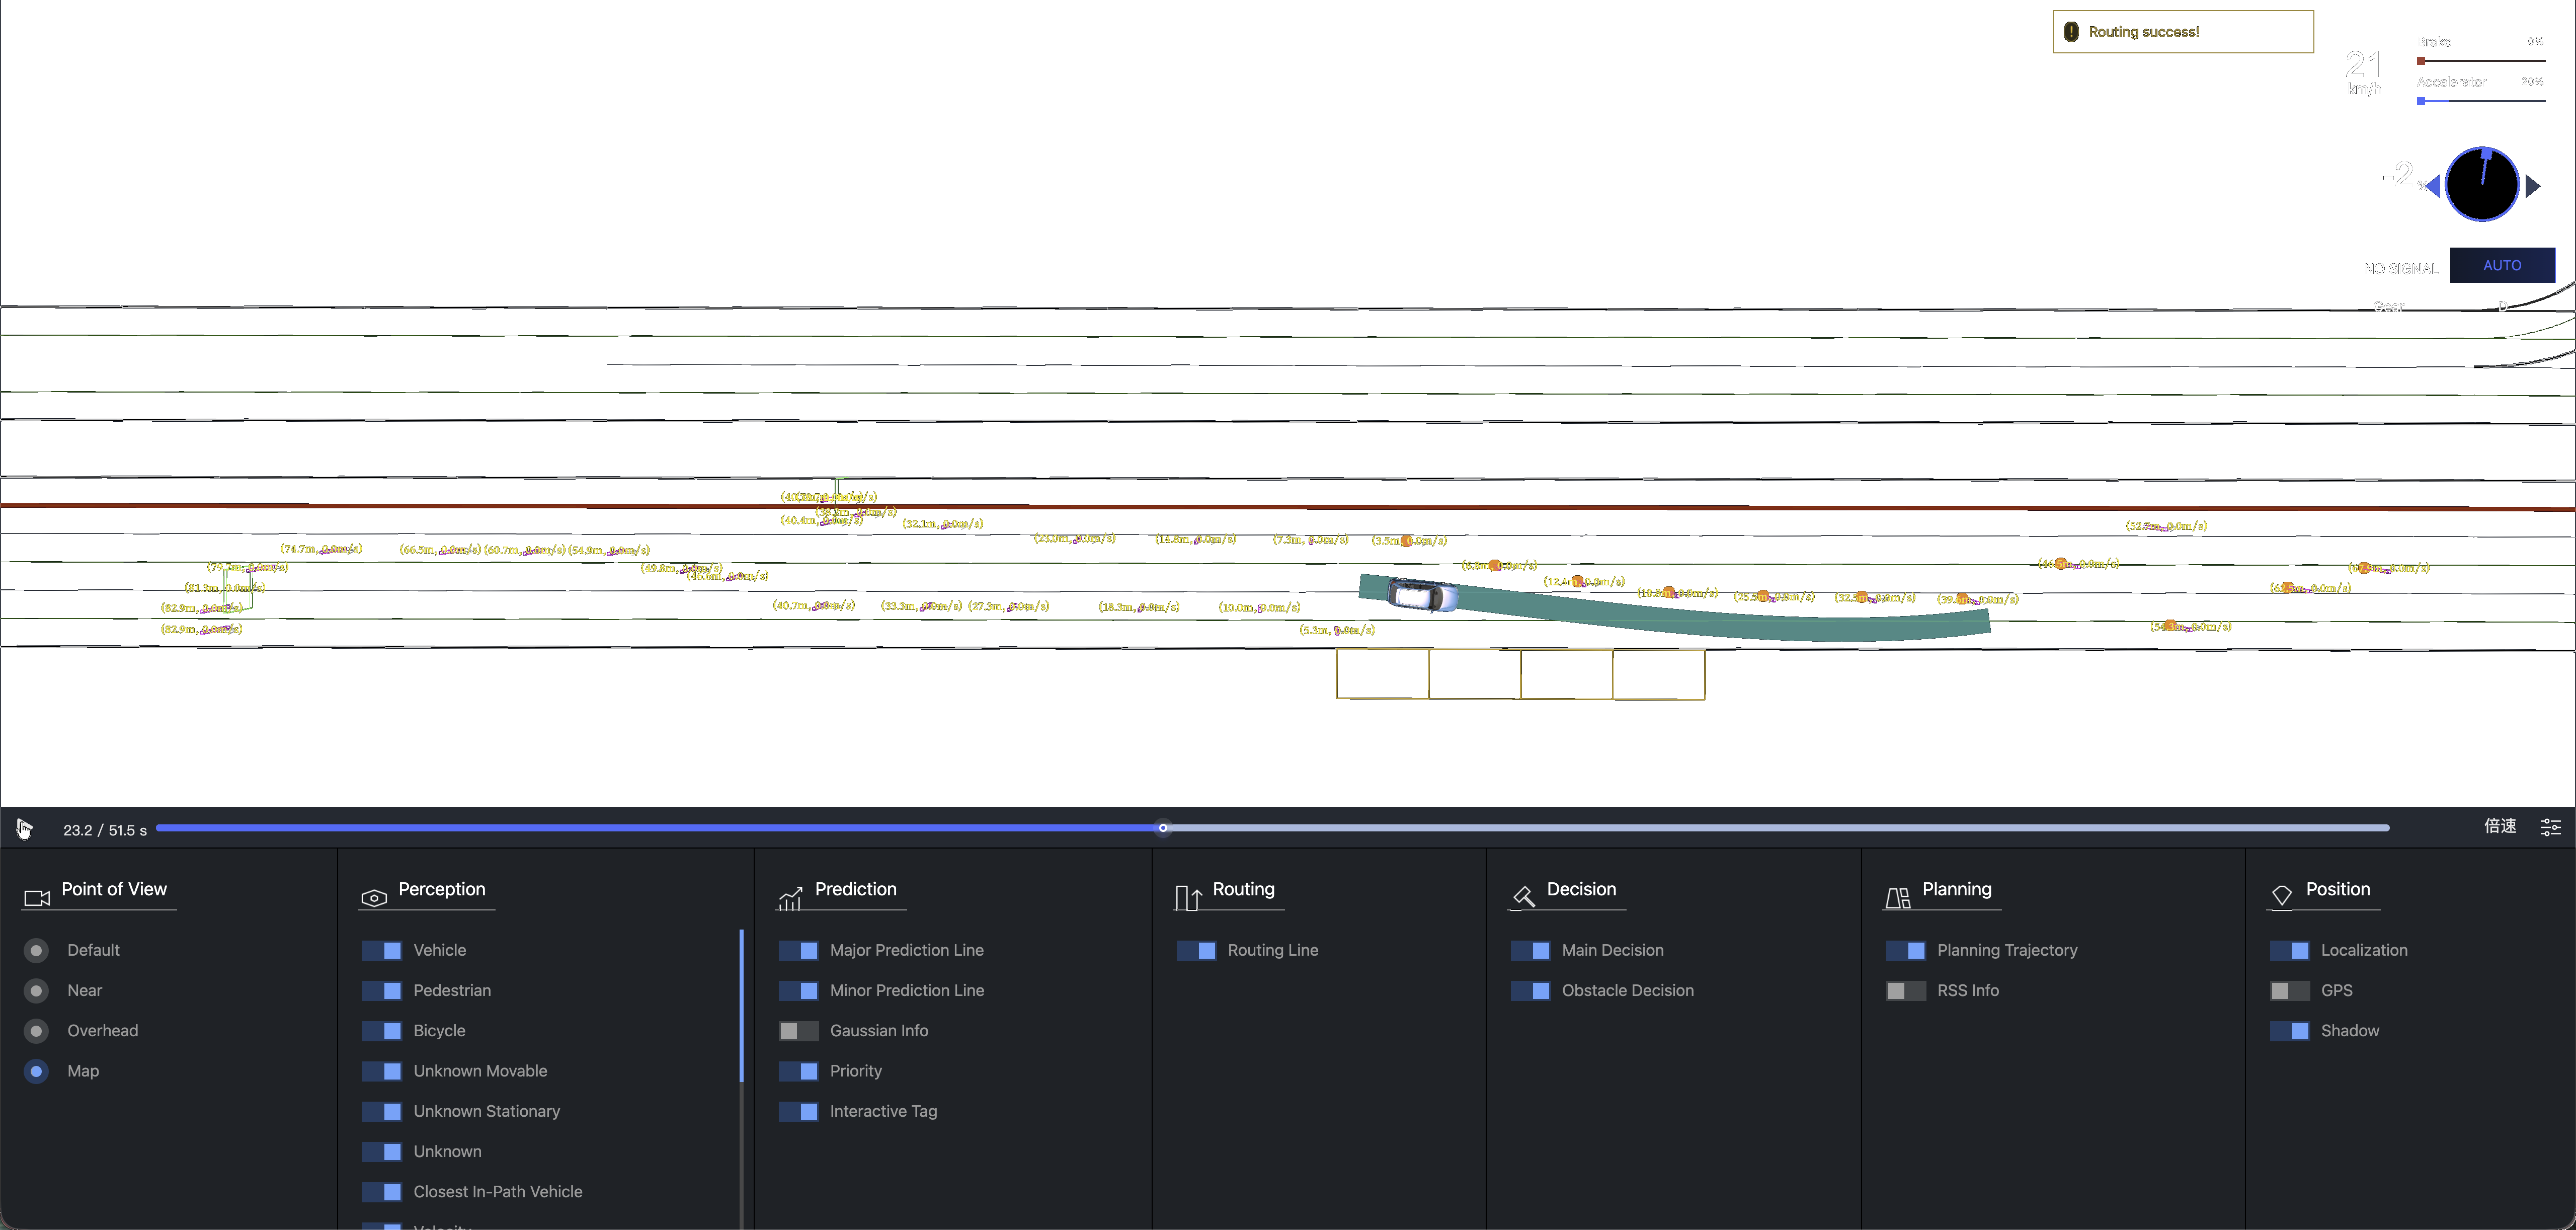
\includegraphics[width=\linewidth]{dreamview/scn03_during.png}\par\vspace{2pt}\footnotesize (c) 单车道绕行\end{minipage}
\caption{Apollo 11.0 Dreamview 中的动态超车（a）、窄通道通行（b）与单车道绕行（c）。}
\label{zh:fig:apollo_cases}
\end{figure}

\section{讨论}
\label{zh:sec:discussion}

\subsection{证据能够确立的内容}

本文的主要结果是约束接口效应，而不是声称某一个优化器支配所有替代方法。MIKU 保留 PVD 求解器，但改变障碍物信息何时以及以何种方式到达求解器。最大收益出现在窄间隙多障碍物和延迟交叉构型中，恰好是预测时域并集或不可逆局部侧向选择会移除可行替代方案的情形。在 B0 已经容易处理的构型中，例如交叉行人和车辆切入类别，总体成功率没有变化。相比所有案例都统一提升，这种结果模式更直接地支持本文提出的机制。

消融实验提供了第二层支持。Top-$K$ 空间同伦和威胁感知裕度解释了总体成功率差异的大部分，而时间同伦图主要在障碍物前后两种通行均可到达时发挥作用。鲁棒占用管在预测噪声下减少碰撞，但相应的进度和加加速度代价表明，面向安全的扩展会消耗可用空间。这些权衡与将可行性、安全性和舒适性视为竞争性运营结果的走廊规划和预测感知规划研究一致 \citep{yoon2024stcorridor,yangbo2023ped,pathspeedstructured2024}。

\subsection{运营含义}

对于基于 PVD 的自动驾驶车辆规划栈，一个可操作的设计规则是在确定路径边界之前保留交互时序，然后将选定的时间语义传递给速度阶段。这样可以在不引入新的下游非线性或混合整数求解器的情况下，减少不必要的兜底停车。该规则尤其适用于窄施工区、临时车道绕行以及多个障碍物共享同一纵向分量的混合交通场景。部署时仍应配备延迟监控器和兜底策略，因为运行时间上尾和不确定性扩展案例仍然具有实际影响。

\subsection{与替代方法的关系}

有限网格参考在小规模比较中取得略高的成功率，但运行时间中位数约高出两个数量级。这一比较说明扩展联合搜索与编译式 PVD 接口之间存在质量—代价权衡，并不能证明 MIKU 在全局上更优。同样，迭代式 B2 基线表明，当缺失信息是已经丢弃的横向类别时，简单重复 PVD 阶段并不足够。因此，MIKU 的贡献在于约束的表示和传递，而不是声称所有部署都不需要迭代或联合搜索。

\subsection{对评估的启示}

3,500 个场景的数值协议、700 个场景的滚动协议和 Apollo 接口案例彼此分开，对于正确解释结果十分重要。第一类估计匹配场景层面的效应，第二类测试重规划下的累积行为，第三类检查工程插入点。将它们合并为一个总分会夸大外部有效性。后续评估应使用公共或道路采集轨迹、与近期外部规划器的匹配比较，并在目标硬件预算下进行原生运行时间测量。

\section{局限性与未来展望}
\label{zh:sec:limitations}

尽管 MIKU 显著增强了多障碍物交通环境下的交互感知约束生成能力，本文方法仍存在若干实际局限，为未来研究指明了方向。

首先，在预测模型与道路几何方面，本文目前的实证评估主要基于结构化道路环境及带有有界噪声包络的恒定速度预测模型。真实交通场景中包含复杂的道路曲率、拓扑交叉口以及周围人类驾驶员的多模态行为不确定性。这一边界在预测误差呈现系统性而非有界性时可能高估碰撞率的降低幅度。后续研究将引入在自然驾驶数据集上训练的校准多模态轨迹预测模型，例如 Trajectron++ 或 MTR，并将区间几何抽象扩展至曲率超过 0.05\,rad/m 的弯道拓扑。

其次，在验证层级方面，当前的实验验证聚焦于大规模数值仿真与 Apollo 11.0 架构内的软件在环测试。后续工作将补充硬件在环时延、传感器处理延迟以及极端天气或退化路面下的底盘动力学，并开展封闭试验场实车测试与通行顺序动态重排下的完备性分析。

\section{结论}
\label{zh:sec:conclusion}

本文提出了面向动态多障碍交通路径—速度规划的 MIKU 交互感知约束重构框架。通过引入到达时间依赖投影、连续群组级侧向划分、威胁感知安全裕度以及时间同伦图，MIKU 在严格保持下游路径和速度二次规划凸优化命题结构完全不变的前提下，系统性地重构了缺失的交互时序与空间拓扑约束接口。此外，固定截面最大间隙定理保证了最优侧向分配可通过 $O(k\log k)$ 扫描高效求解，消除了传统多障碍物分配中的指数级组合爆炸。

在覆盖七类典型交通构型的 3,500 个配对仿真场景中，实证评估表明 MIKU 将无碰撞到达目标率从 62.7\% 显著提升至 77.5\%，相对基线提升 14.8 个百分点，并将碰撞率从 2.2\% 减半至 1.1\%。性能增益在极具挑战的狭窄通道提升 65.4 个百分点，在延迟交叉场景提升 26.8 个百分点，直接证实了重构后的约束接口能够有效消除虚假死锁。消融实验证实群组级侧向协调与威胁感知裕度构筑了空间可行走廊的基础，而时间同伦图则有效解析了因果通行时序。算法完整规划周期的中位时延仅为 9.98 ms，充分满足自动驾驶典型控制周期的硬实时要求。

在 Apollo 11.0 架构内的软件在环验证进一步证实，MIKU 无需改动原生二次规划求解器即可无缝接入量产级自动驾驶系统，在动态超车、窄通道与车道绕行等代表性工况下表现出优异的兼容性与避障平滑性。闭环滚动重规划实验亦验证了多周期动态行驶下的轨迹一致性与鲁棒性。后续研究将把该框架拓展至校准的多模态轨迹预测、复杂立体弯道道路网络以及全系统实车在环测试平台。

\section*{数据可用性声明}
匿名复现实验包包含冻结的场景生成器、配置文件、聚合结果、原始行以及分析脚本。论文录用后，该复现实验包将存入 Zenodo 或同等长期保存的公共仓库，分配 DOI，并以 CC BY 4.0 许可发布。在审稿期间，编辑部可基于合理请求获取上述材料。

\section*{代码可用性声明}
复现正文数值表所需的分析与评估脚本已包含在补充材料压缩包中。论文录用后，完整的 MIKU 规划器代码及其 Apollo 11.0 集成文件将在公开的 GitHub 仓库中发布，并归档至 Zenodo 分配 DOI，采用 Apache-2.0 许可，以与上游 Apollo 项目保持兼容。补充材料压缩包本身仅包含用于复现所报告数值表的脚本；完整的集成文件将在录用时随公开仓库一并发布。

\section*{基金}
\ifdefined\anonymousversion
本研究获得公共科研计划的资助；资助单位与项目编号将在录用版本中恢复。资助方未参与研究设计、数据采集、分析或发表决策。
\else
本研究得到襄阳市异构大数据市级重点实验室、湖北省优势特色学科群``新能源汽车与智慧交通''以及湖北省重点研发计划项目编号 2025BEB002 的支持。
\fi

\section*{利益披露声明}
作者声明本文不存在需要披露的竞争性利益。

\section*{伦理声明}
本研究未涉及人类受试者、人体数据或动物实验。全部评测均基于仿真场景以及针对 Apollo 11.0 的软件在环接口测试，因此无需正式的伦理审批与知情同意程序。

\section*{发表同意声明}
不适用；本文未涉及任何个体数据。

\section*{作者贡献}
\ifdefined\anonymousversion
作者贡献依据 CRediT 分类体系，涵盖概念化、方法、软件、形式化分析、数据整理、验证、调查、可视化、论文初稿撰写、论文审阅与编辑、监督、项目管理以及基金获取。各作者的具体角色将在录用版本中恢复。
\else
JiaWang Liao：概念化、方法、软件、形式化分析、数据整理、可视化以及论文初稿撰写。YuFei Hu：方法、验证、调查以及论文审阅与编辑。ChaoYang Shi：软件、验证、调查、可视化以及论文审阅与编辑。ChengJiao Sun：监督、项目管理、基金获取、概念化以及论文审阅与编辑。全体作者均审阅并批准最终稿件。
\fi

\section*{AI 使用声明}
\ifdefined\anonymousversion
OpenAI Codex GPT-5 于 2026 年 9 月访问，用于将作者已有的中文稿翻译、文字编辑并按期刊呈现需要重组。该工具未用于原创或得出科学论证，也未用于生成底层数据或分析。引用选择和书目信息已根据作者的原始材料及正式记录核验。作者已查阅适用的工具使用条款，确认这种使用适合发表，并对全文内容的原创性、完整性和准确性，包括参考文献的准确性，承担全部责任。一位署名的合作者在非匿名版本中注明，其审阅并核验了完整的英文稿，包括全部科学主张、公式、引用和数值结果。
\else
OpenAI Codex GPT-5 于 2026 年 9 月访问，用于将作者已有的中文稿翻译、文字编辑并按期刊呈现需要重组。该工具未用于原创或得出科学论证，也未用于生成底层数据或分析。引用选择和书目信息已根据作者的原始材料及正式记录核验。JiaWang Liao 对完整的英文稿进行了审阅与核验，包括全部科学主张、公式、引用和数值结果。作者已查阅适用的工具使用条款，确认这种使用适合发表，并对全文内容的原创性、完整性和准确性，包括参考文献的准确性，承担全部责任。
\fi



\bibliographystyle{apacite}
\bibliography{references}

\end{document}
